\vspace{1cm}
\begin{center}
    \Huge{\textbf{\underline{Exercise 2}}}
\end{center}

\vspace{0.45cm}

\begin{center}
    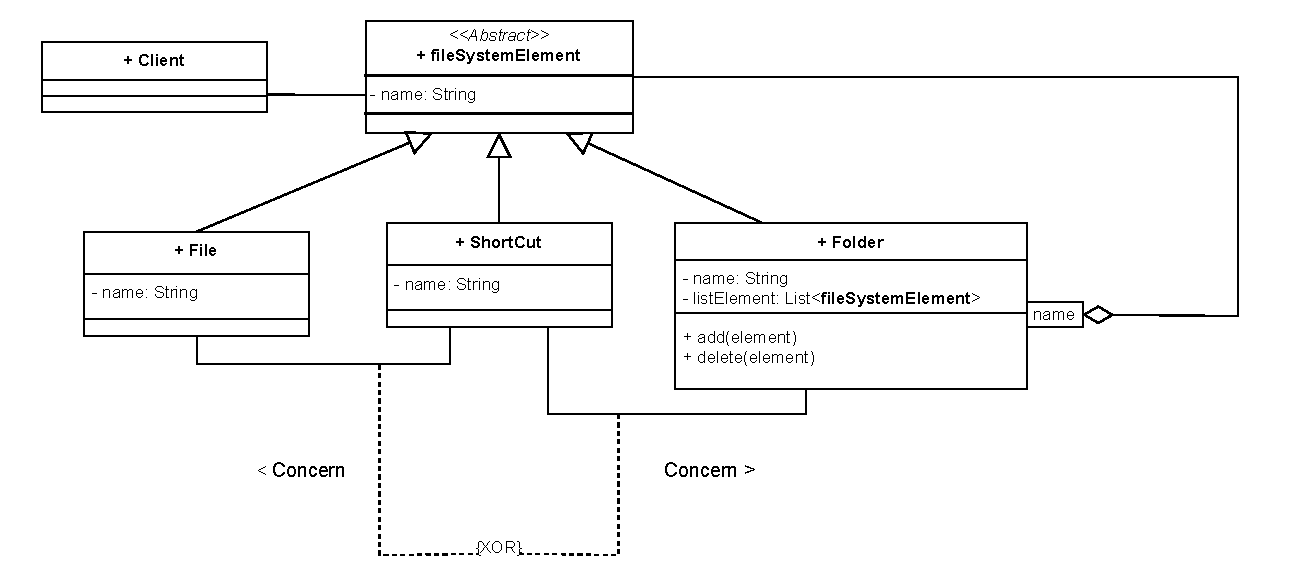
\includegraphics[height=0.22\textheight]{Exercices/EX2/ex2.drawio.pdf}
\end{center}

\vspace{0.25cm}
\begin{prettyBox}{Explication}{myblue}
We used the \textbf{composite design pattern} because the file system is inherently nested and recursive: 
we have \texttt{shortcut} and \texttt{file} as the leaf elements, and \texttt{folder} as the complex nesting element.\\[0.15cm]
A folder can contain either leaf elements or other folders, forming a hierarchical structure.\\[0.15cm] 
A \texttt{shortcut} can be associated with either a file or a folder, but never both at the same time 
this exclusivity is why we used the XOR (exclusive OR) operator.
\end{prettyBox}

